% Appendix D, Figure D.5 --- "The dodecahedral POVM, end to end".  The layout only.
%
% Layout: card_oct_body.tex's header is binding.  Deviations from it, and only
% they, are listed here.
%
%   * THIS IS THE BINDING CARD, at 21.30pt of reserve: its float is the
%     tallest of the five against \textheight = 700.50687pt.  Every literal
%     in the generator's emitters is shared across the five, so any wording
%     change must be re-measured here before it ships.
%   * the ray line is the most fragile object on the five pages: ten rays,
%     443.86pt natural at \small against the 452.9679pt line -- 9.11pt of
%     slack.  Re-measure before changing any ray label.
%   * band 1 nests the worked $E_1$ under the two vertex blocks, as on the
%     icosahedron.
%   * band 2 runs 377pt + 75pt, with $B$ and $C$ in the side column; the
%     unfactored $A$ is the chapter head's (assertion 32).
%   * band 4's draw note runs to TWO lines, and every word of it is
%     measured.  "Realization forces the $\TwoI$ draw." alone is false: the
%     ten-word coin times a drawn $\{\Id, X, Y, Z\}$ flip, applied last, puts
%     forty non-group elements on both of randomness's jobs at once,
%     exactly, for half the $\Phi$ (randomized_twojobs' check_flip_completion),
%     so "forces" needs its scope ("Among groups") and the cheaper draw needs
%     saying.  The relabelling "($X$ or $Y$ swaps the pair)" may not be
%     dropped either: without the swap the four flips average the readout to
%     a multiple of $\Id$.  The wrapping is NOT read off the natural width:
%     888.29pt breaks to three lines where 880.80 still sets two, because
%     $\Id, X, Y, Z$ and $0.4\,\Phi$ cannot break.  Set the candidate in a
%     \vtop at 452.9679pt and read its DEPTH -- 2.5pt is one line, about
%     14pt is two.  A third line costs about 11pt of the reserve, so
%     re-measure before adding a word; if height is ever needed the ladder
%     below is the source.  One thing the note must not say: that a $\TwoT$
%     draw would hand this card the inscribed cube.  A $\TwoT$ draw splits
%     the ten axes 4 + 6 and the ALIGNMENT VERTEX selects which -- vertex 9,
%     this card's, selects the six, not the inscribed cube.
%   * the cut ladder, if this card must ever give height, in measured order:
%     drop the worked $E_1$ (-25.34pt); band rules 4.00 -> 3.00pt (-4.00pt);
%     the six \NIS 5 -> 4pt (-6.00pt); the key's `upper`/`lower` heads
%     (-11pt, at the cost of head 3 naming the wires again); and only as a
%     last resort \PanelScale 2.47 -> 2.20 here alone (-17pt), which forfeits
%     the uniform panel this design spends most on.
% All macros below are \def and therefore local to the figure environment.
\parindent=0pt \parskip=0pt
% Auto-generated by code/_build_povm_cards.py -- DO NOT EDIT.
% The data blocks of the dodecahedral card of Appendix D
% (paper/figures/card_dodec_body.tex \input's this and calls them).  Every
% number is derived from code/data/*.npz, Decker's circuits as
% randomized_decker rebuilds them, Figure 1.1's own \RecipeSeriesStrip, and
% Tables E.1, 5.2, D.1, D.3 and D.4, and is checked back against them before
% this file is written; see the builder's docstring for the checks (and
% _povm_cards_controls.py, which shows each of them failing on one corrupted
% literal: 100 negative controls, all aborting, 0 stale).
% Requires: booktabs, mathtools, hyperref, and the thesis macros \Id, \pmat,
% \bra, \ket, \braket, \Tr, \C, \sigmavec, \TwoT, \TwoO, \TwoI, \phig,
% \invphig, \sigmaz.  The body defines \NIS, \CTR, \PBOX, \COL, \FULLHEAD,
% \BANDRULE and \TAB, which \CardSide and the tables use.
% Regenerate with `cd code && uv run _build_povm_cards.py`.

\newcommand{\CTitle}{The dodecahedral POVM, end to end}
\newcommand{\CPtrStrip}{Introduction reference: Figure~\ref{fig:tetrahedron-recipe}}
\newcommand{\CHeadA}{Vertices and effects, $E_k = \tfrac1V(\Id + \hat n_k \cdot \sigmavec)$.}
\newcommand{\CPtrA}{Table~\ref{tab:povm-atlas} $\cdot$ Equation~\eqref{eq:povmform}}
\newcommand{\CHeadB}{Circuit; the dashed $U_g$ is an optional prepended rotation.}
\newcommand{\CPtrB}{Section~\ref{subsec:rotated-povms} $\cdot$ Table~\ref{tab:decker-pose}}
\newcommand{\CHeadC}{Register $\to$ vertex, top wire first; --- never fires}
\newcommand{\CPtrC}{Table~\ref{tab:decker-labels} $\cdot$ Section~\ref{sec:decker:using}}
\newcommand{\CHeadD}{Coin over axes, no ancilla, $\ket0$-vertex first, rightmost factor first}
\newcommand{\CPtrD}{Table~\ref{tab:decker-vs-coin} $\cdot$ Section~\ref{subsec:randomized-implementations} $\cdot$ Table~\ref{tab:binary-icosahedral-group-2i}}

\newcommand{\CStrip}{{\footnotesize\setlength{\tabcolsep}{4pt}\renewcommand{\arraystretch}{0.88}%
\begin{tabular}{@{}c c c c l l l@{}}
\toprule
$V$ & group & anc. & dead & reorientation exact? & relabelling & \hyperref[tab:decker-vs-coin]{coin over axes}\\
\midrule
20 & $\TwoI$ & 4 & 12 & no thesis gate set & permuted & 10 axes, 4 with one $\Phi$\\
\midrule
\multicolumn{7}{@{}l@{}}{only the octahedral coin is exact --- this dilation is not (Theorem~\ref{thm:main}, Appendix~\ref{sec:decker:exactness})}\\
\bottomrule
\end{tabular}}}

\newcommand{\CardVertexBlockA}{%
\begin{tabular}{@{}r l r@{}}
\toprule
$k$ & $\hat n_k$\ $(\times\tfrac{1}{\sqrt3})$ & $\bra{0}E_k\ket{0}$ \\
\midrule
$1$ & $(+1,\,+1,\,+1)$ & $0.0789$ \\
$2$ & $(+1,\,+1,\,-1)$ & $0.0211$ \\
$3$ & $(+1,\,-1,\,+1)$ & $0.0789$ \\
$4$ & $(+1,\,-1,\,-1)$ & $0.0211$ \\
$5$ & $(-1,\,+1,\,+1)$ & $0.0789$ \\
$6$ & $(-1,\,+1,\,-1)$ & $0.0211$ \\
$7$ & $(-1,\,-1,\,+1)$ & $0.0789$ \\
$8$ & $(-1,\,-1,\,-1)$ & $0.0211$ \\
$9$ & $(\phantom{+}0,\,+\invphig,\,+\phig)$ & $0.0967$ \\
$10$ & $(\phantom{+}0,\,+\invphig,\,-\phig)$ & $0.0033$ \\
\bottomrule
\end{tabular}
}

\newcommand{\CardVertexBlockB}{%
\begin{tabular}{@{}r l r@{}}
\toprule
$k$ & $\hat n_k$\ $(\times\tfrac{1}{\sqrt3})$ & $\bra{0}E_k\ket{0}$ \\
\midrule
$11$ & $(\phantom{+}0,\,-\invphig,\,+\phig)$ & $0.0967$ \\
$12$ & $(\phantom{+}0,\,-\invphig,\,-\phig)$ & $0.0033$ \\
$13$ & $(+\invphig,\,+\phig,\,\phantom{+}0)$ & $0.0500$ \\
$14$ & $(+\invphig,\,-\phig,\,\phantom{+}0)$ & $0.0500$ \\
$15$ & $(-\invphig,\,+\phig,\,\phantom{+}0)$ & $0.0500$ \\
$16$ & $(-\invphig,\,-\phig,\,\phantom{+}0)$ & $0.0500$ \\
$17$ & $(+\phig,\,\phantom{+}0,\,+\invphig)$ & $0.0678$ \\
$18$ & $(+\phig,\,\phantom{+}0,\,-\invphig)$ & $0.0322$ \\
$19$ & $(-\phig,\,\phantom{+}0,\,+\invphig)$ & $0.0678$ \\
$20$ & $(-\phig,\,\phantom{+}0,\,-\invphig)$ & $0.0322$ \\
\bottomrule
\end{tabular}
}

\newcommand{\CIdent}{$\sum_k E_k = \Id$, $\Tr E_k = \tfrac1{10}$, rank one, a $5$-design; numbered at each axis's near vertex.}
\newcommand{\CIdentB}{$E_1 = \tfrac1{20}\pmat{1+1/\sqrt3 & (1-i)/\sqrt3 \\ (1+i)/\sqrt3 & 1-1/\sqrt3}$, $E_{g(k)} = U_g E_k U_g^\dagger$.}

\newcommand{\CParams}{$U_R = R_{\hat y}(-\arccos(\phig/\sqrt{\phig+2}))$ inverts Table~\ref{tab:decker-pose}'s $R$; a drawn $U_g$ twirls and relabels outcomes by $g^{-1}$.\par\vskip1pt $A^\dagger$: Equation~\eqref{eq:adagger}; $A$: Equation~\eqref{eq:aunfactored}\par\vskip1pt $u_\pm = \sqrt{1/2 \pm \phig/(2\sqrt3)}$, $v_\pm = \mp\sqrt{1/2 \pm 1/(2\sqrt{2+\phig})}$, each $\pm1$ in the two rotation boxes is $\pm\sqrt{1/2}$\par\vskip1pt $Q_{32}^\dagger$: the CNOT $\ket{00000}\mapsto\ket{00000}$, $\ket{01001}\mapsto\ket{00001}$; $\mathsf{F}_5^\dagger \oplus I_3$, lower three wires\par\vskip1pt $\tilde{M}_{32}^\dagger = (A^\dagger \otimes (\mathsf{F}_5^\dagger \oplus I_3))\,Q_{32}^\dagger$, the Naimark extension unitary the solid box implements}

\newcommand{\CardSide}{\CTR{\hsize}{$B = \pmat{u_- & -u_+ \\ u_+ & u_-}$}\NIS{4pt}\CTR{\hsize}{$C = \pmat{v_- & v_+ \\ v_+ & -v_-}$}}

\newcommand{\CardKey}{%
\begin{tabular}{@{}c c c c c c c c c@{}}
\toprule
& \multicolumn{8}{c}{\footnotesize lower} \\
{\footnotesize upper} & $\mathtt{000}$ & $\mathtt{001}$ & $\mathtt{010}$ & $\mathtt{011}$ & $\mathtt{100}$ & $\mathtt{101}$ & $\mathtt{110}$ & $\mathtt{111}$ \\
\midrule
$\mathtt{00}$ & 17 & 3 & 11 & 9 & 1 & --- & --- & --- \\
$\mathtt{01}$ & 20 & 6 & 10 & 12 & 8 & --- & --- & --- \\
$\mathtt{10}$ & 18 & 14 & 7 & 5 & 13 & --- & --- & --- \\
$\mathtt{11}$ & 19 & 15 & 2 & 4 & 16 & --- & --- & --- \\
\bottomrule
\end{tabular}
}

\newcommand{\CKappa}{Run $U_R$ and read the key, or skip $U_R$ and read Decker's own numbered list~\cite{decker2004quantumcircuitssinglequbit}: either way $\kappa = 1$, free. His circuit with our list, index for index, is the mismatch: $\kappa = -0.009703$; under the drawn twirl it costs a $1/\kappa^2 = 10621.86\times$ premium in shots, never a bias.}

\newcommand{\CRays}{$\Phi$~$1$,\,$8$ $\cdot$ $\mathbf{F}^\dagger \Phi$~$2$,\,$7$ $\cdot$ $\Phi^\dagger \mathbf{F}^\dagger$~$3$,\,$6$ $\cdot$ $\Phi^\dagger$~$5$,\,$4$ $\cdot$ $\Id$~$9$,\,$12$ $\cdot$ $\mathbf{Z}$~$11$,\,$10$ $\cdot$ $\mathbf{F}$~$13$,\,$16$ $\cdot$ $\mathbf{F} \mathbf{X}$~$14$,\,$15$ $\cdot$ $\mathbf{F}^\dagger$~$17$,\,$20$ $\cdot$ $\mathbf{F}^\dagger \mathbf{Z}$~$19$,\,$18$}

\newcommand{\CCoin}{Draw one, apply it, then the alignment ($9 \mapsto \hat z$, inexact); measure $Z$. Among groups, realization forces $\TwoI$. With a drawn flip $\Id, X, Y, Z$ last ($X$ or $Y$ swaps the pair), these forty twirl too, at $0.4\,\Phi$, not $\TwoI$'s $0.8$.}

\long\def\NIS#1{\vskip #1\nointerlineskip}
\long\def\CTR#1#2{\hbox to #1{\hss #2\hss}}
\long\def\PBOX#1#2{\vtop{\hsize=#1\parindent0pt\sloppy\emergencystretch=1.5em\small #2}}
\long\def\COL#1#2{\vtop{\hsize=#1\parindent0pt\hbox{}\nointerlineskip #2}}
\long\def\FULLHEAD#1#2#3{\hbox to \hsize{\small\textbf{#1}\,#2\hfil{\footnotesize #3}}}
\def\BANDRULE{\vskip2pt\hrule height0.5pt\vskip1.5pt\nointerlineskip}
\long\def\TAB#1{{\small\renewcommand{\arraystretch}{0.88}\setlength{\tabcolsep}{3pt}#1}}
%
\vbox{\hsize\textwidth\parindent0pt
%
% --- title and the header strip: Figure 1.1's own row -----------------------
\hbox to \hsize{\large\bfseries \CTitle\hfil{\normalfont\footnotesize \CPtrStrip}}%
\NIS{5pt}%
\hbox{\CStrip}%
\BANDRULE
%
% --- band 1: the object -----------------------------------------------------
\FULLHEAD{1}{\CHeadA}{\CPtrA}%
\NIS{5pt}%
\hbox to \hsize{%
  \COL{170pt}{\CTR{170pt}{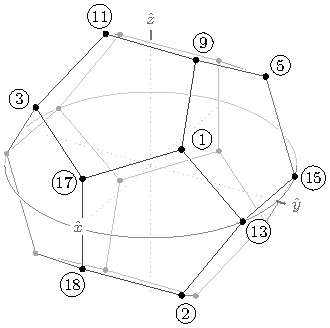
\includegraphics{figures/card_dodec_sphere.pdf}}}%
  \hfil
  \COL{277pt}{\hbox to 277pt{\hfil\TAB{\CardVertexBlockA}\hskip10pt\TAB{\CardVertexBlockB}}%
    \NIS{4pt}\PBOX{277pt}{\CIdentB}}%
}%
\NIS{4pt}%
\PBOX{\hsize}{\CIdent}%
\BANDRULE
%
% --- band 2: the machine ----------------------------------------------------
\FULLHEAD{2}{\CHeadB}{\CPtrB}%
\NIS{5pt}%
\hbox to \hsize{%
  \COL{377pt}{\hbox to 377pt{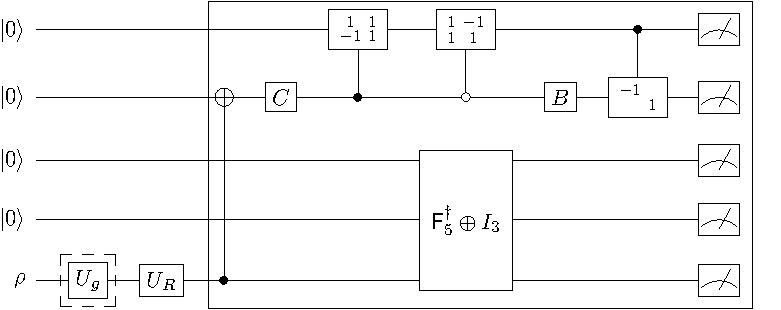
\includegraphics{figures/card_dec_dodec.pdf}\hss}}%
  \hfil
  \COL{75pt}{\small\CardSide}%
}%
\NIS{5pt}%
\PBOX{\hsize}{\CParams}%
\BANDRULE
%
% --- band 3: the readout ----------------------------------------------------
\FULLHEAD{3}{\CHeadC}{\CPtrC}%
\NIS{5pt}%
\hbox to \hsize{%
  \COL{206pt}{\TAB{\CardKey}}%
  \hfil
  \COL{238pt}{\PBOX{238pt}{\CKappa}}%
}%
\BANDRULE
%
% --- band 4: the alternative ------------------------------------------------
\FULLHEAD{4}{\CHeadD}{\CPtrD}%
\NIS{5pt}%
\PBOX{\hsize}{\CRays}%
\NIS{2pt}%
\PBOX{\hsize}{\CCoin}%
}%
